%----------------------------------------------------------------------------------------
%	PACKAGES AND THEMES
%----------------------------------------------------------------------------------------
\documentclass[aspectratio=169,xcolor=dvipsnames]{beamer}
\usepackage[english,russian]{babel}
\usetheme{Simple}

\usepackage{hyperref}
\usepackage{graphicx} % Allows including images
\usepackage{booktabs} % Allows the use of \toprule, \midrule and \bottomrule in tables

%----------------------------------------------------------------------------------------
%	TITLE PAGE
%----------------------------------------------------------------------------------------

% The title
\title{Анализ эффективности нейросетевых вычислений с учетом аппаратных возможностей платформ}
\subtitle{Курсовая работа}

\author[Pin-Yen] {Бинцаровский Леонид Петрович}
\institute[NTU] % Your institution may be shorthand to save space
{
    % Your institution for the title page
    Белорусский государственный университет\\
    ФПМИ, ДМА, 3 курс\\
    руководитель: старший преподаватель Пирштук Д. И.
    \vskip 3pt
}
\date{Минск, 2024} % Date, can be changed to a custom date


%----------------------------------------------------------------------------------------
%	PRESENTATION SLIDES
%----------------------------------------------------------------------------------------

\begin{document}

\begin{frame}
    % Print the title page as the first slide
    \titlepage
\end{frame}

% \begin{frame}{Overview}
%     % Throughout your presentation, if you choose to use \section{} and \subsection{} commands, these will automatically be printed on this slide as an overview of your presentation
%     \tableofcontents
% \end{frame}

%------------------------------------------------
\section{First Section}
%------------------------------------------------

\begin{frame}{Применение замены фона на видеопотоке}
    \begin{itemize}
        \item Рекламные материалы
        \item Графический дизайн
        \item Игры и симуляторы
        \item Увлекательные видеоролики
        \item Видеозвонки
    \end{itemize}
\end{frame}

%------------------------------------------------

\begin{frame}{Методы сегментации изображения и виды предобученных моделей}
    \begin{enumerate} 
      \item Выделение краёв;
      \item Методы разреза графа;
      \item Сегментация с помощью предобученной модели:
        \begin{enumerate} 
            \item \textbf{Semantic segmentation};
            \item \textbf{Hair segmentation};
            \item \textbf{Multi-class segmentation};
            \item \textbf{Instance segmentation}.
        \end{enumerate} 
    \end{enumerate}
\end{frame}

%------------------------------------------------

\begin{frame}{Постановка задачи}
    Для реализации задачи обработки видеопотока с заменой фона, будут использоваться:

    \begin{block}{Модель для сегментации}
        Semantic segmentation
    \end{block}

    \begin{block}{Фреймворк}
        MediaPipe
    \end{block}

    \begin{block}{Язык программирования, среда разработки и операционная система}
        С++, Visual Studio и Windows
    \end{block}
\end{frame}

%------------------------------------------------

\begin{frame}{Основные элементы конвейера}
    \begin{columns}[c] % The "c" option specifies centered vertical alignment while the "t" option is used for top vertical alignment

        \column{.45\textwidth} % Left column and width
        \begin{figure}[h]
            \center{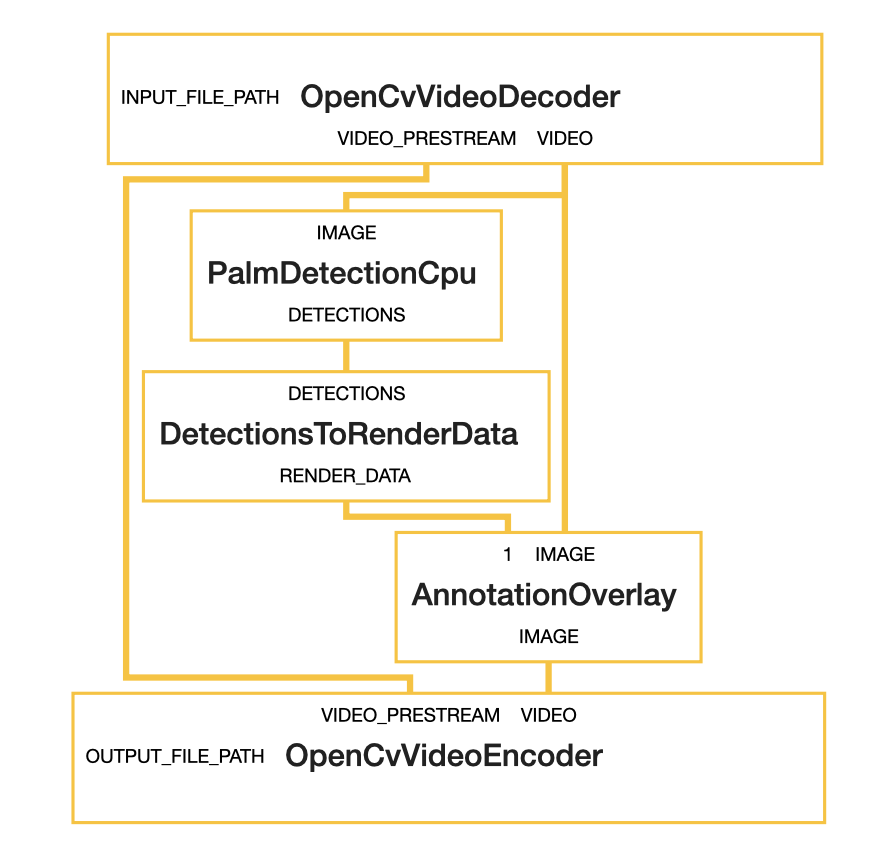
\includegraphics[width=0.9\linewidth]{images/graph.png}}
            \label{ris:subgraph}
        \end{figure}

        \column{.5\textwidth} % Right column and width
        \begin{enumerate}
            \item Пакет (Packet)
            \item Узлы (Nodes or calculator)
            \item Потоки (Streams)
            \item Подграф (Subgraph)
            \item Граф (Graph)
        \end{enumerate}

    \end{columns}
\end{frame}

%------------------------------------------------
\section{Second Section}
%------------------------------------------------

\begin{frame}{Реализация архитектуры конвейера}
    В ходе разработки конвейера был реализован граф Selfie\_segmentation\_cpu\_ultimate.pbtxt:
    \begin{figure}[h]
        \center{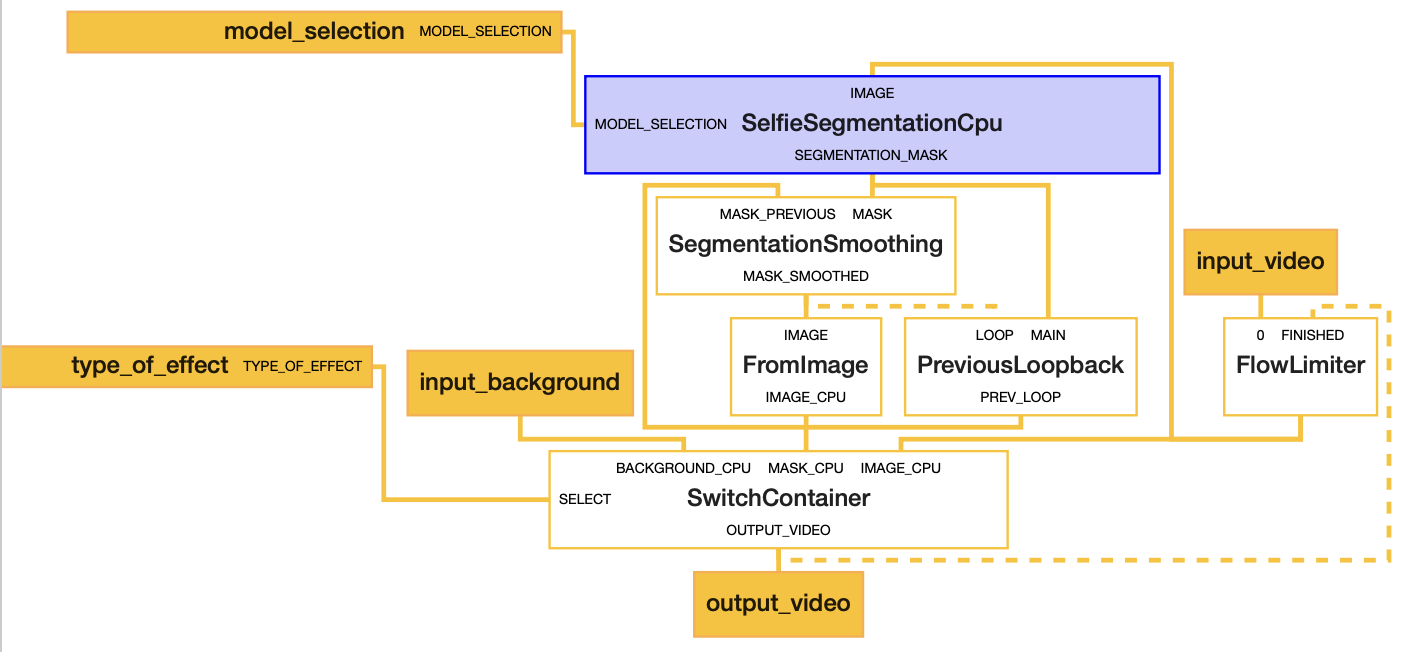
\includegraphics[width=0.7\linewidth]{images/doneGraph.png}}
        \label{ris:subgraph}
    \end{figure}
\end{frame}

\begin{frame}{Реализация архитектуры конвейера}
    А также подграф Selfie\_segmentation\_cpu.pbtxt:
    \begin{figure}[h]
        \center{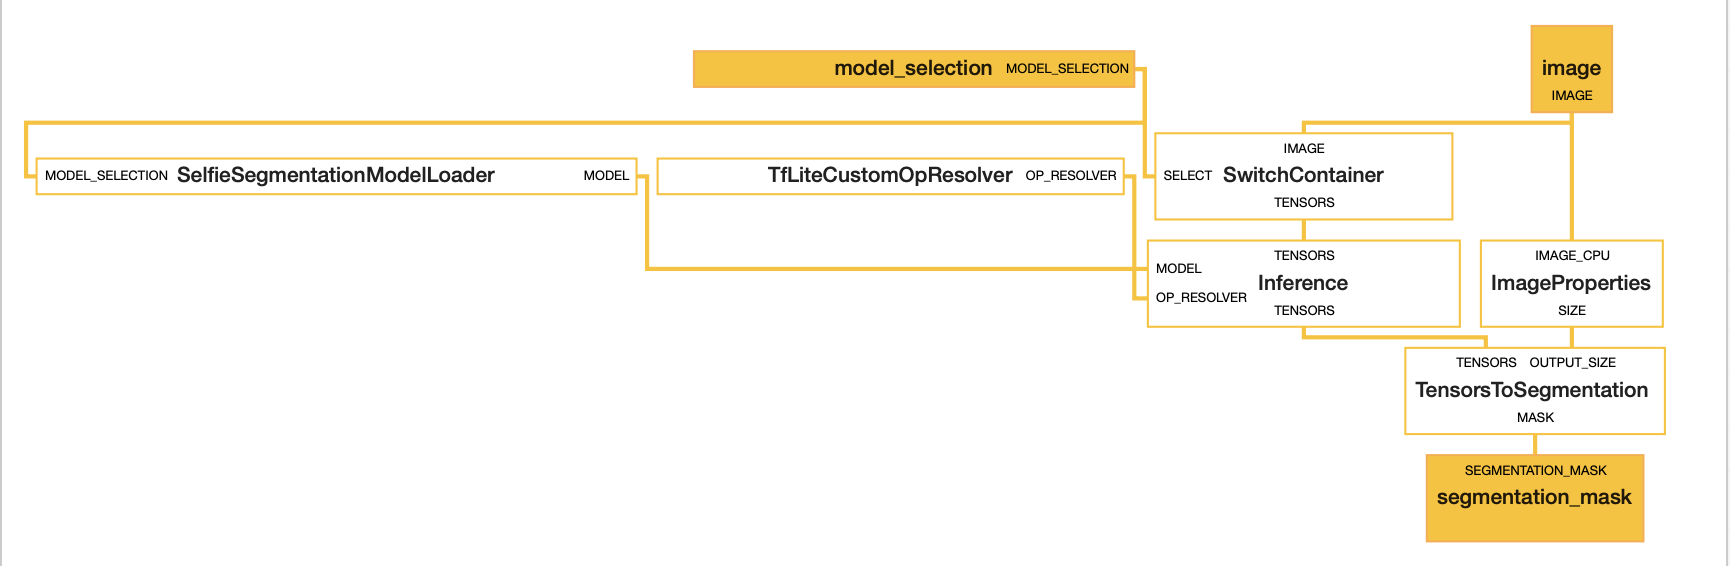
\includegraphics[width=0.7\linewidth]{images/subgraph.png}}
        \label{ris:subgraph}
    \end{figure}
\end{frame}

%------------------------------------------------

\begin{frame}{Реализация калькуляторов}
    Калькулятор представляет собой класс С++, реализующий интерфейс CalculatorBase. В данном классе обязательно присутствуют следующие функции:
    \begin{enumerate}
        \item \textbf{::mediapipe::Status GetContract(CalculatorContract* cc)};
        \item \textbf{::mediapipe::Status Process(CalculatorContext* cc)};
        \item \textbf{::mediapipe::Status Open(CalculatorContext* cc)};
    \end{enumerate}
    
    Помимо самого кода калькулятора необходимо определить proto-файл с конфигурацией калькулятора.
\end{frame}

%------------------------------------------------

\begin{frame}{Реализация классов для работы в среде Visual Studio}
    \begin{columns}[c] % The "c" option specifies centered vertical alignment while the "t" option is used for top vertical alignment

        \column{.45\textwidth} % Left column and width
        \begin{figure}[h]
            \center{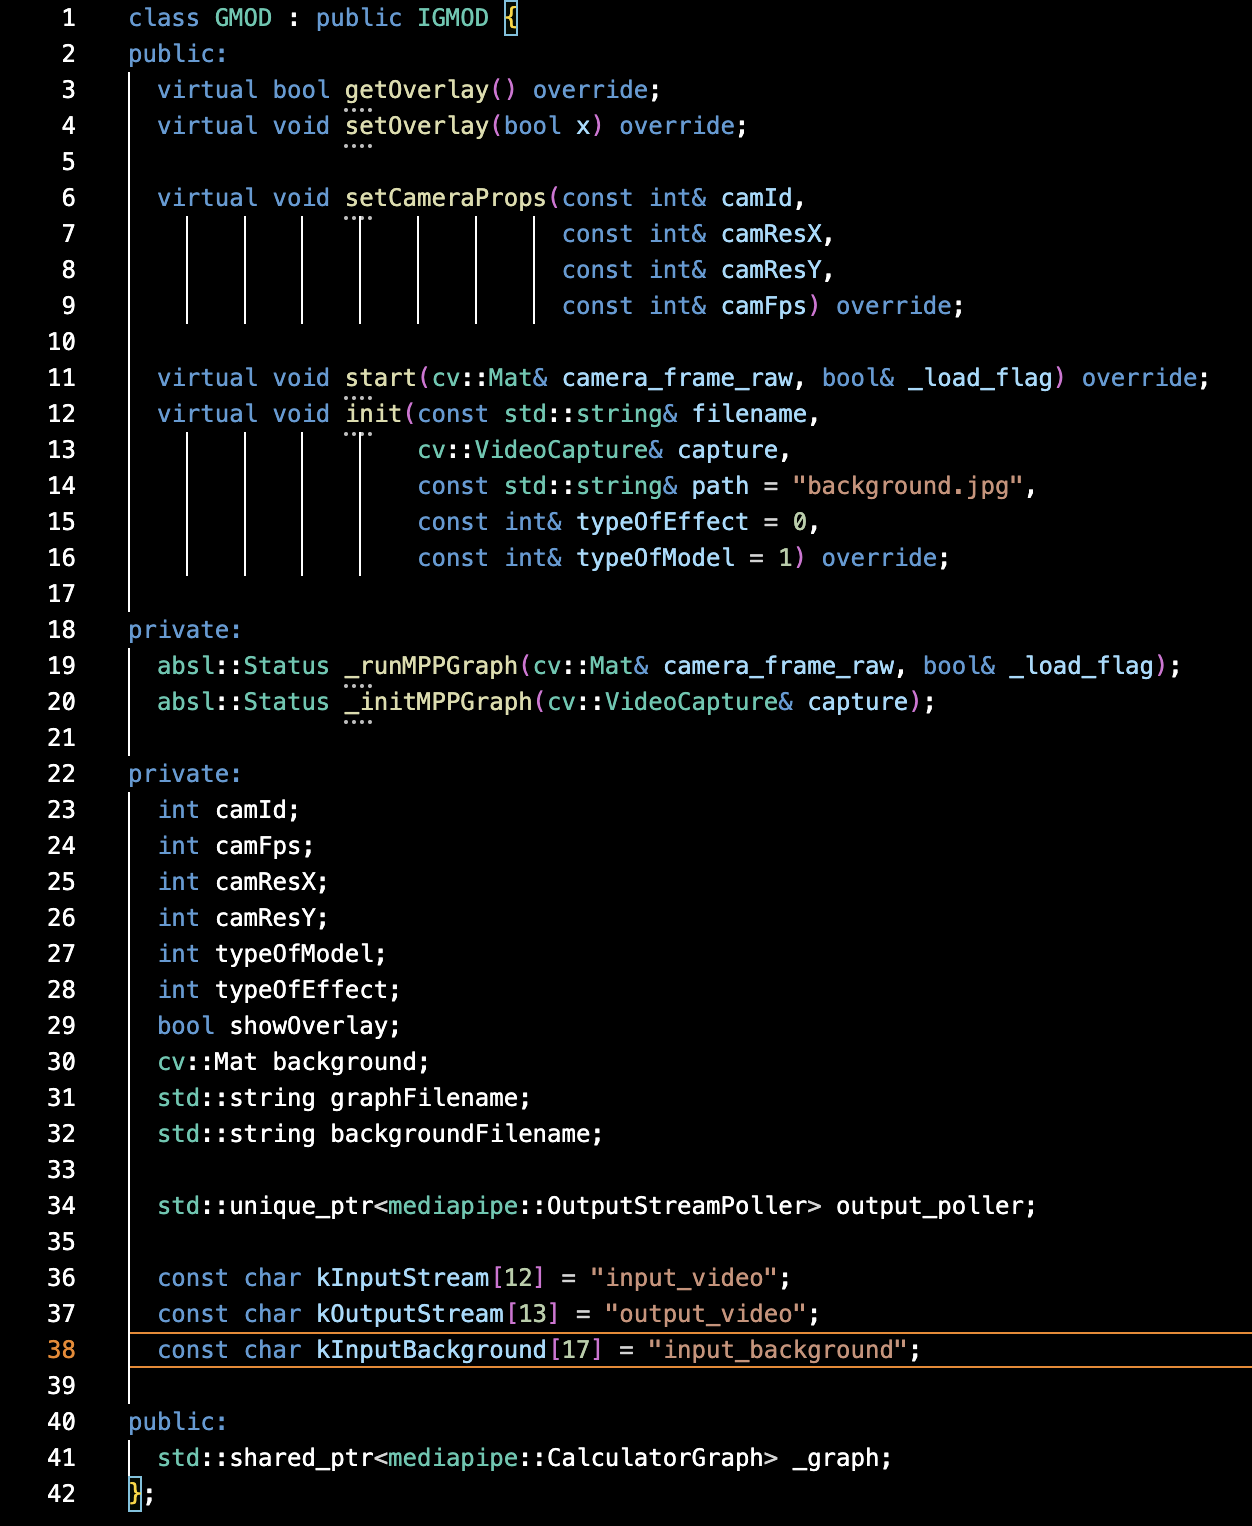
\includegraphics[width=0.8\linewidth]{images/class.png}}
            \label{ris:subgraph}
        \end{figure}

        \column{.5\textwidth} % Right column and width
        В большинстве своем в фреймворке MediaPipe используются макросы, которые возвращают ошибки типа absl::Status из фреймворка MediaPipe и их нельзя обработать напрямую в коде программы в Visual Studio. Поэтому были реализованы вспомогательные функции в private, выполняющие основной функционал, и основные функции (будут вызываться в основной программе), которые являются обертками функций из private и обрабатывают возможные ошибки.

    \end{columns}
\end{frame}

%------------------------------------------------

\begin{frame}{Результат работы}
    \begin{figure}[h]
        \center{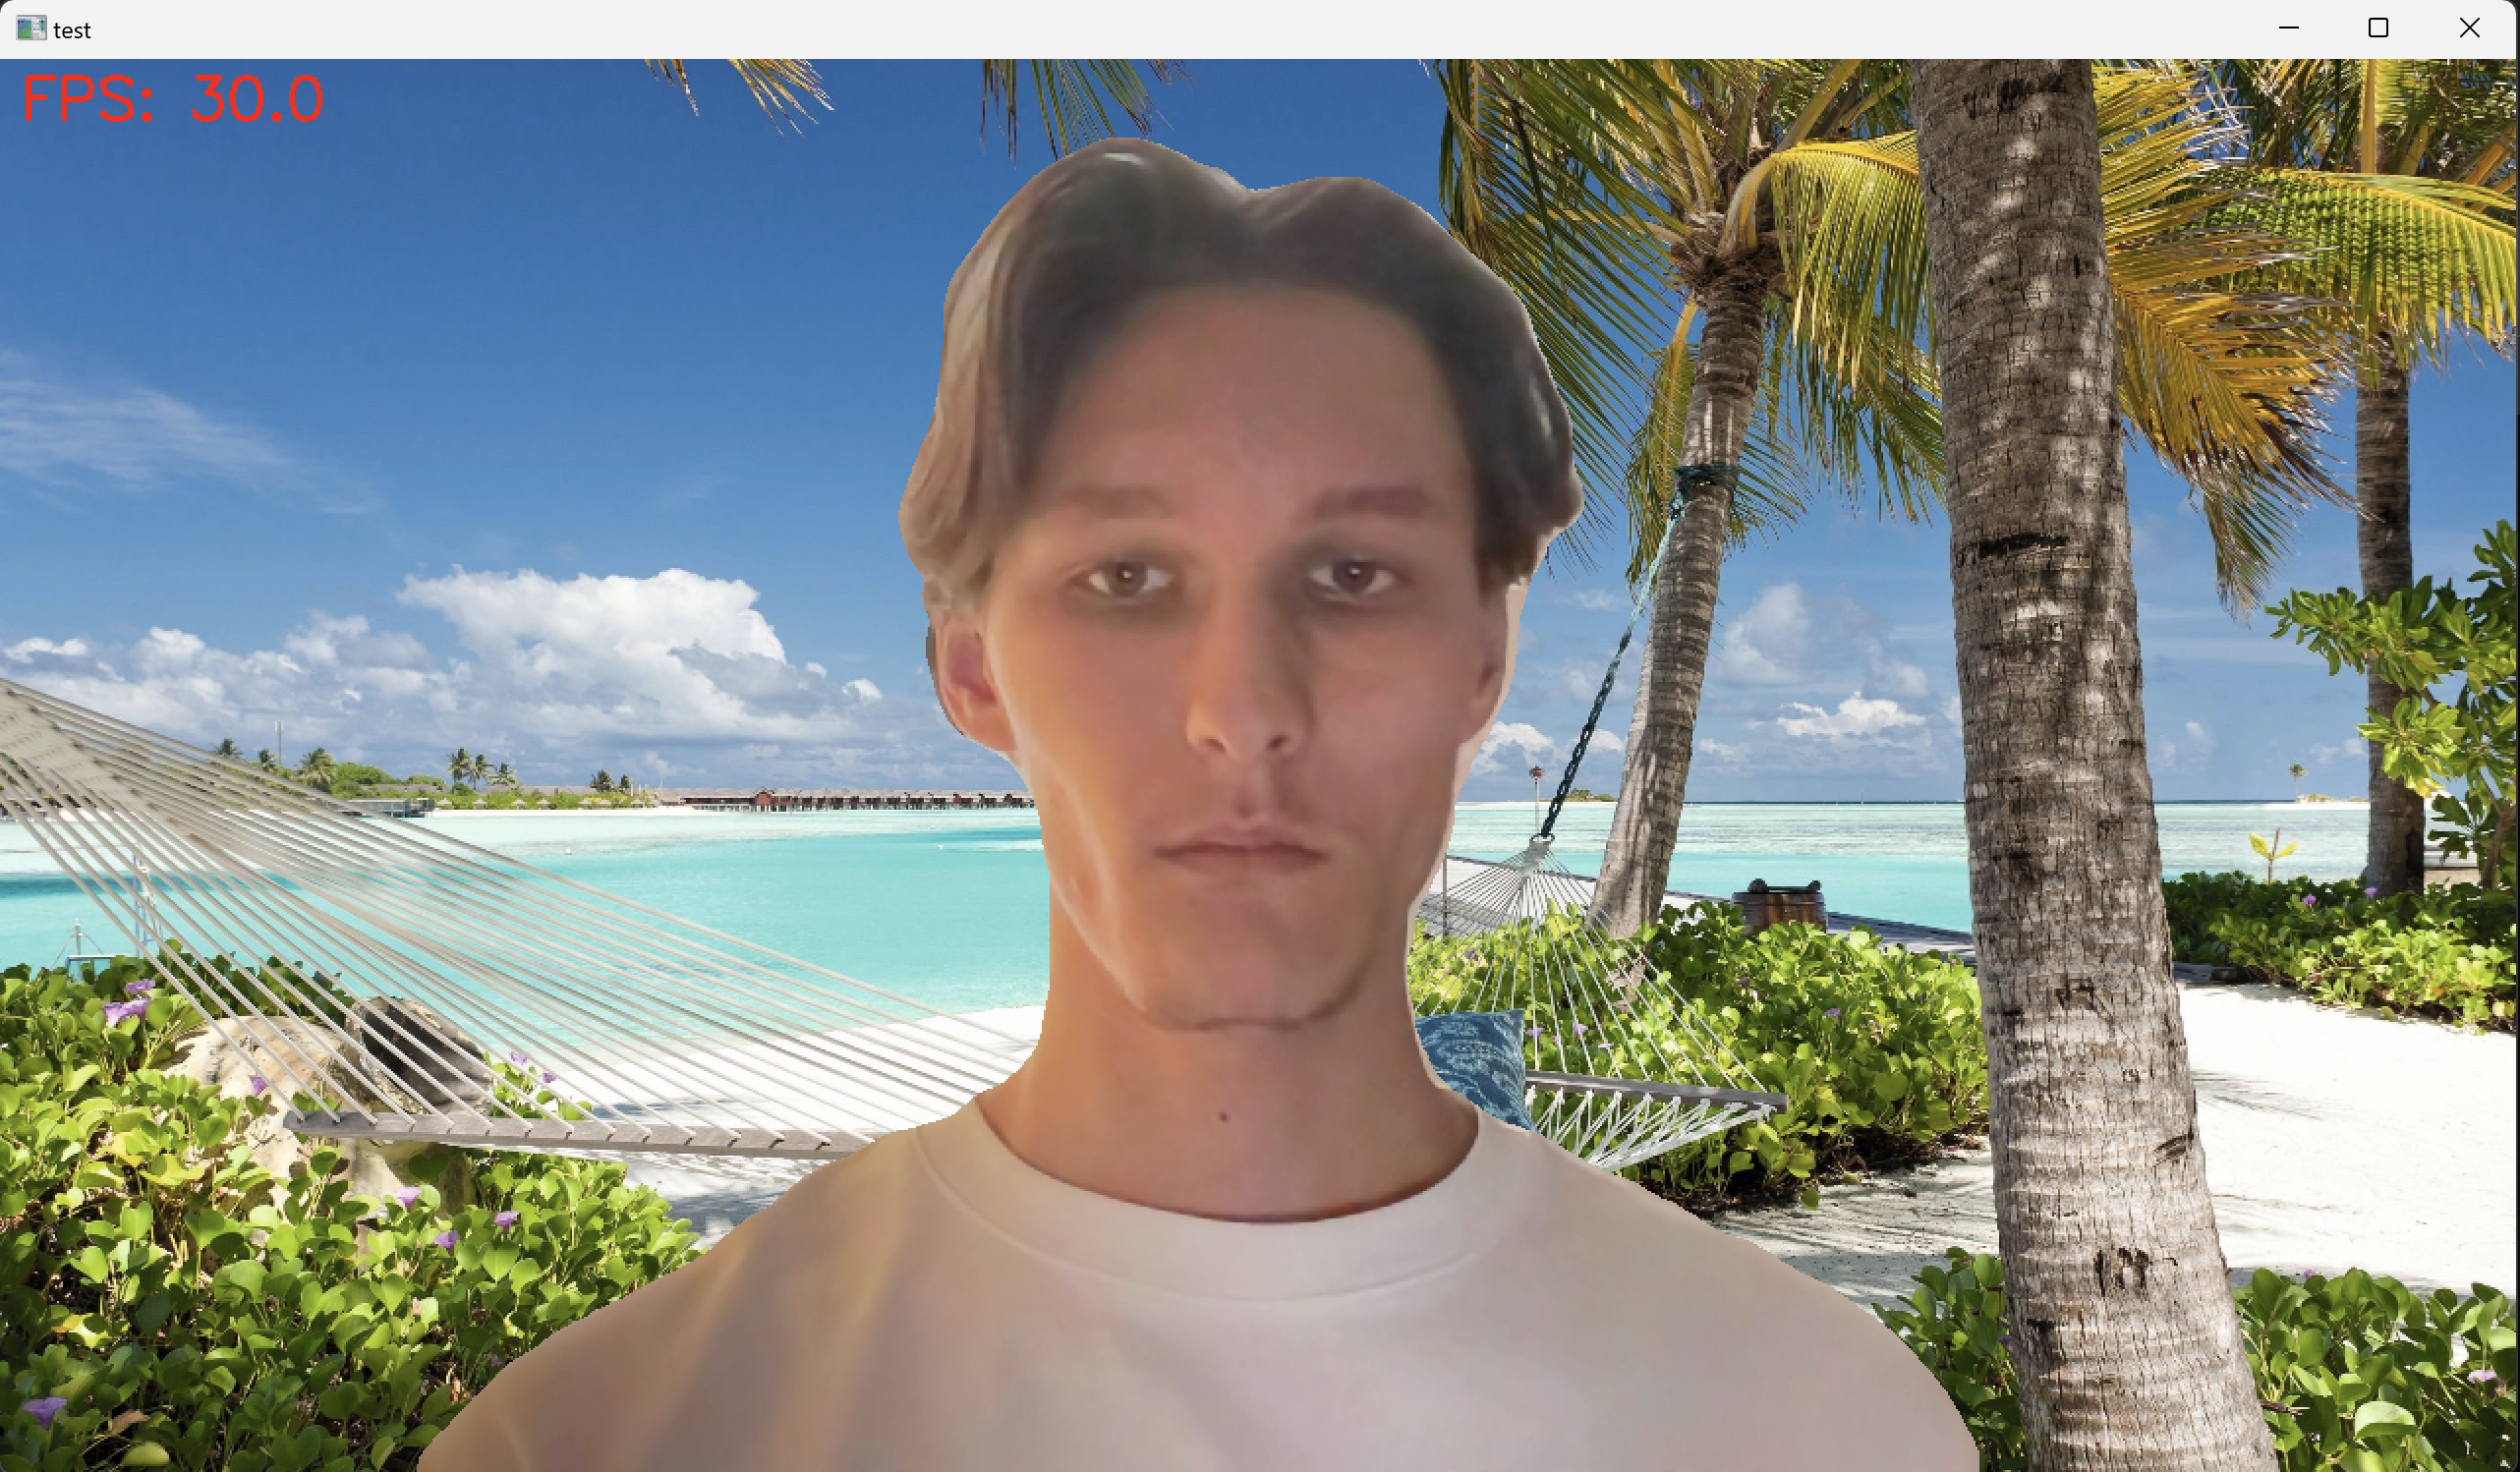
\includegraphics[width=0.7\linewidth]{images/test.png}}
        \label{ris:subgraph}
    \end{figure}
\end{frame}

%------------------------------------------------

\begin{frame}{Выводы}
    \begin{itemize}
        \item Была рассмотрена задача обработки видеопотока с помощью фреймворка MediaPipe, а также ее применение на прикладном уровне;
        \item Сделан краткий обзор фреймворка MediaPipe;
        \item Выполнен обзор основных элементов конвейера фреймворка MediaPipe;
        \item Резработана архитектура ковейера и реализованы необходимые калькуляторы для него;
        \item Реализованы классы для работы с фреймфорком MediaPipe в среде разработки Visual Studio;
        \item Успешно протестированы результаты работы.
    \end{itemize}
\end{frame}

%----------------------------------------------------------------------------------------

\end{document}